\section{Analysis of Social Network}\label{analysis-of-social-network}

\subsection{Objectives}\label{objectives}

The data from Social Network will be indexed in Graph Database, then
data mining techniques will be implemented and some predictions will be
extracted. Based on a paper, the first analysis will be the user
engagement in posts of a branch page. The focus is understand the
analysis model and reproduce on GDB.

\subsection{Workflow}\label{workflow}

\begin{figure}
\centering
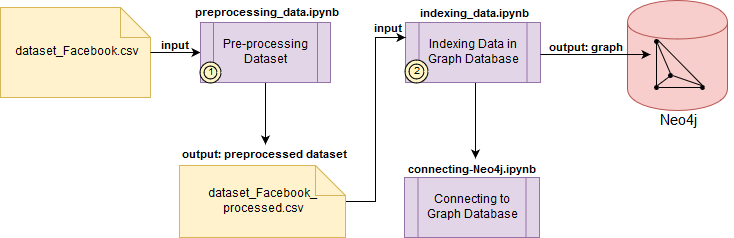
\includegraphics{../figures/research.png}
\caption{Research Workflow}
\end{figure}

\subsection{Description of data}\label{description-of-data}

The dataset used is available in
http://archive.ics.uci.edu/ml/datasets/Facebook+metrics. The dataset has
19 features and 500 instances.

\subsection{Methods}\label{methods}

Neo4j Graph Database will be used in this research. Neo4j has librarys
to be used in Python.

\subsection{References}\label{references}

S. Moro, P. Rita and B. Vala. Predicting social media performance
metrics and evaluation of the impact on brand building: A data mining
approach. Journal of Business Research, Elsevier, In press, 2016.
